\section{Kapitel 7}
\subsection{Aufgabenstellung}
Wie sollen 7 Klassen Definieren, dabei sollen wir uns überlegen welche davon Instanziierbar sind und welche
nicht. Anschlie\ss end soll jede Klasse sinnvolle Methoden und Attribute enthalten.

\subsection{Anforderungsdefinition}
\begin{enumerate}
	\item Definiere folgende Klassen: Viereck, konvexes Viereck, Trapez, Parallelogramm, Rhombus, Rechteck, Quadrat
	\item Definiere sinnvolle Methoden und Attribute
\end{enumerate}

\subsection{Entwurf}
Für den Entwurf wurde ein Klassendiagramm angefertigt. Wobei hier die Klasse Viereck Abstrakt ist und
die Wesentlichen Methoden beinhaltet. Beim Konvexen Viereck werden die wesentlichen Attribute eines 
Vierecks definiert, dazu auch deren Berechnung. Zudem muss hier auch die Methode für den 
Flächeninhalt und Umfang überschrieben werden. Das Trapez erbt vom Konvexen Viereck, Parallelogramm
vom Trapez, Rhombus vom Parallelogramm, Rechteck von Parallelogramm ud Quadrat vom Rechteck. 
\begin{center}
	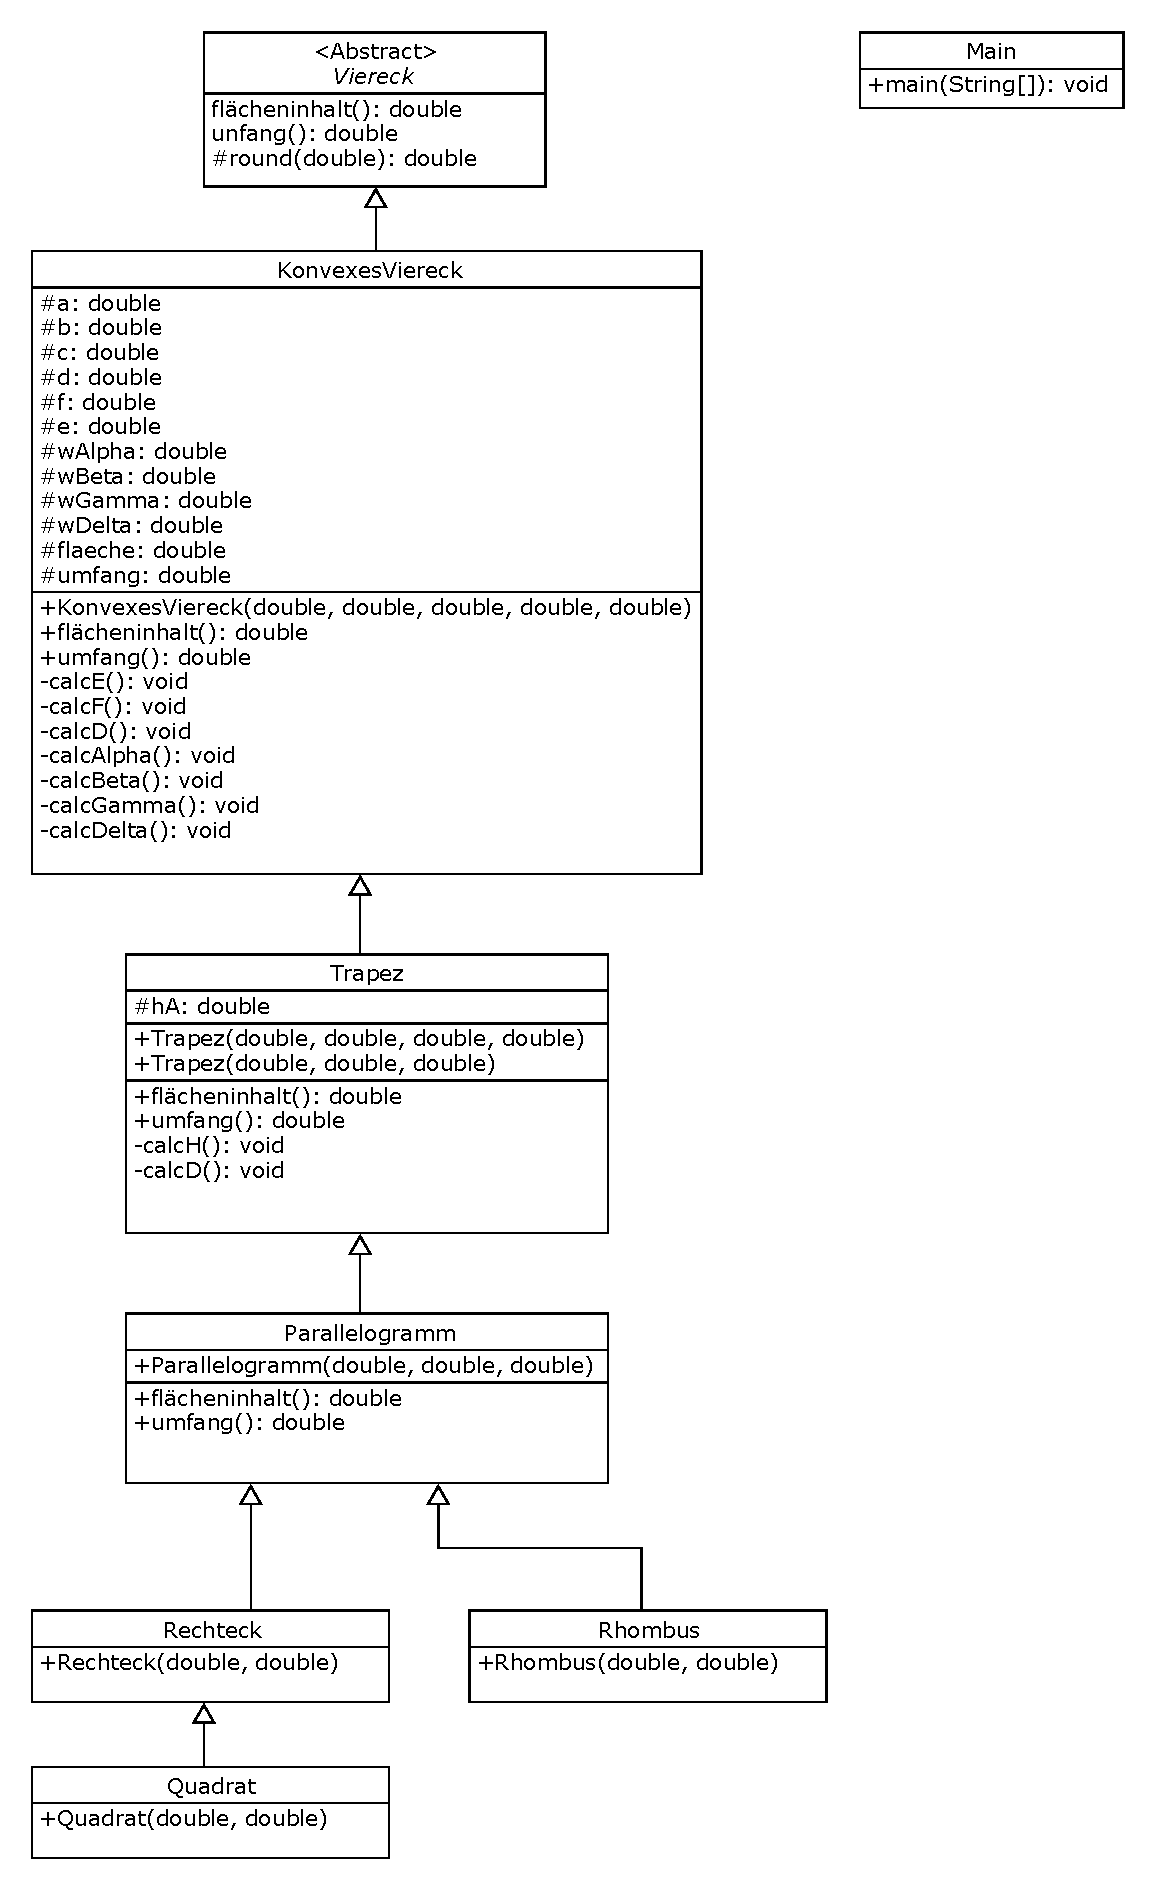
\includegraphics[width=0.95\textwidth]{uml/uml_c7_p1.pdf}
\end{center}

\subsection{Quelltext}
\subsubsection{Main.java}\
\lstinputlisting[language = Java , frame = trBL , escapeinside={(*@}{@*)}]{../chapter_07/src/main/java/chapter_07/Main.java}
\subsubsection{Viereck.java}\
\lstinputlisting[language = Java , frame = trBL , escapeinside={(*@}{@*)}]{../chapter_07/src/main/java/chapter_07/figures/Viereck.java}
\subsubsection{KonvexesViereck.java}\
\lstinputlisting[language = Java , frame = trBL , escapeinside={(*@}{@*)}]{../chapter_07/src/main/java/chapter_07/figures/KonvexesViereck.java}
\subsubsection{Trapez.java}\
\lstinputlisting[language = Java , frame = trBL , escapeinside={(*@}{@*)}]{../chapter_07/src/main/java/chapter_07/figures/Trapez.java}
\subsubsection{Parallelogramm.java}\
\lstinputlisting[language = Java , frame = trBL , escapeinside={(*@}{@*)}]{../chapter_07/src/main/java/chapter_07/figures/Parallelogramm.java}
\subsubsection{Rhombus.java}\
\lstinputlisting[language = Java , frame = trBL , escapeinside={(*@}{@*)}]{../chapter_07/src/main/java/chapter_07/figures/Rhombus.java}
\subsubsection{Rechteck.java}\
\lstinputlisting[language = Java , frame = trBL , escapeinside={(*@}{@*)}]{../chapter_07/src/main/java/chapter_07/figures/Rechteck.java}
\subsubsection{Quadrat.java}\
\lstinputlisting[language = Java , frame = trBL , escapeinside={(*@}{@*)}]{../chapter_07/src/main/java/chapter_07/figures/Quadrat.java}

\subsection{Testdokumentation}


\subsection{Benutzungshinweise}


\subsection{Anwendungsbeispiel}
Nach dem man das Programm gestartet hat, sollte folgende Ausgabe erscheinen:
\begin{lstlisting}[frame = trBL , escapeinside={(*@}{@*)}]
	[sebastian@laptop bin]$ java Main
	223.2733105547887 2808.779545976002
	35.17638090205041 49.99999999999999
	50.0 120.0
	32.0 45.256
	30.0 50.0
	20.0 25.0
	[sebastian@laptop bin]$ 
\end{lstlisting}